\newpage
\section{Durchführung}
\label{sec:Durchfuehrung}
Der Versuch ist in 4 Teilmessungen aufgeteilt.
Im ersten Teil des Versuchs wird die Zeitabhängigkeit der Amplitude untersucht.
Um diese Zeitabhängigkeit festzustellen wird eine Rechtecksschwingung über einen Wiederstand $R_1$ ,eine Spule $L$ und einen Kondensator $C$ gesendet (\ref{fig:Aufbau1}).
Mit dem Ozilloskop wird die Spannung über dem Kondensator abgenommen und das Bild des Oszilloskops wird abfotografiert (\ref{fig:bild1}) und analysiert.
\begin{figure}
    \centering
    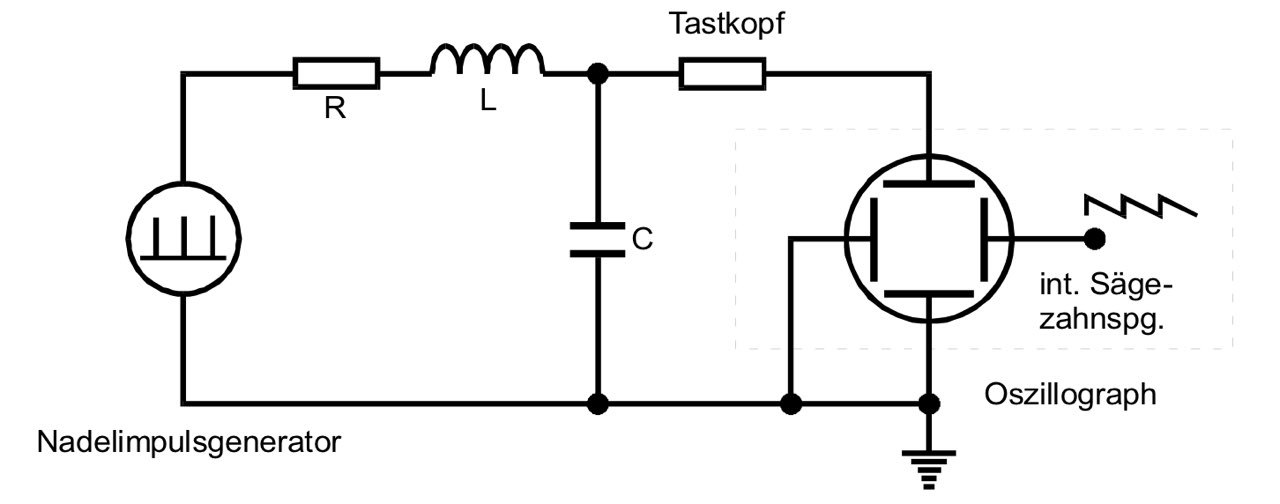
\includegraphics[width=0.6\textwidth]{bilder/Zeitabhaengigkeit_Amplitude.jpeg}
    \caption{Versuchsaufbau - Zeitabhängigkeit der Amplitude}
    \label{fig:Aufbau1}
\end{figure}

Im zweiten Teil des Versuchs soll der Grenzwiederstand $R_{ap}$ bestimmt werden bei dem der aperiodische Grenzfall eintritt.
Dazu wird der gleiche Aufbau wie für den ersten Teil verwendet, allerdings wird nun ein regelbarer Wiederstand verwendet (\ref{fig:Aufbau1}).\\

Im dritten Teil des Versuchs wird die Frequenzabhängigkeit der Kondensatorspannung an einem Serienresonanzkreis gemessen.
Der Serienresonanzkreis ist eine Schaltung bei der  der Generator ein Sinussignal durch den größeren der beiden Wiederstande $R_2$, durch die Spule $L$ und durch einen Kondensator $C$ leitet (\ref{fig:Aufbau2}).
Wieder wird das Signal parallel zum Kondensator abgenommen um die Spannung zu messen.
Für die Messung wird zuerst die Frequenz bestimmt bei der die höchste Spannung gemessen wird, bei Schaltkasten 3 lag diese Frequenz ungefähr bei $f = 35 \text{kHz}$.
Nun werden jeweils 7 ganzzahlige Werte unter und über dieser Frequenz eingestellt und die entsprechende Spannung abgelesen.
\begin{figure}
    \centering
    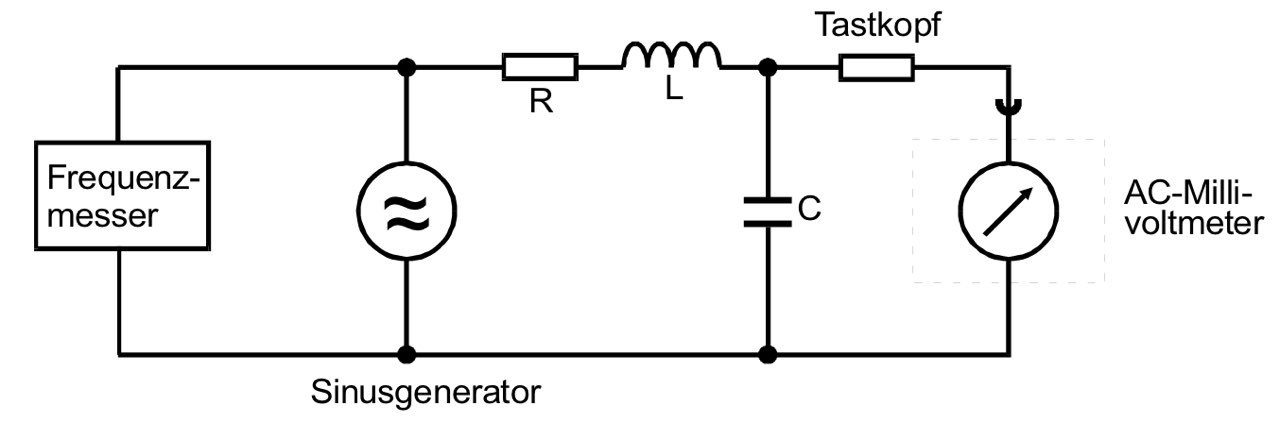
\includegraphics[width=0.6\textwidth]{bilder/Frequenzgang_RLC.jpeg}
    \caption{Versuchsaufbau - Frequenzabhängigkeit der Spannung}
    \label{fig:Aufbau2}
\end{figure}

Im vierten Teil des Versuchs wird die Abhängigkeit der Phase (zwischen Erreger- und Kondensatorspannung) von der Frequenz bestimmt.
Es wird die Kondensatorspannung wie in Teil drei des Versuchs gemessen und zusatzlich wird noch das Erregersignal abgenommen und im Oszilloskop dargestellt(\ref{fig:Aufbau3}).
Anhand der 2 Kurven im Oszilloskop kann der Phasenunterschied durch den Abstand der Minima der Kurven abgelesen werden.

\begin{figure}
    \centering
    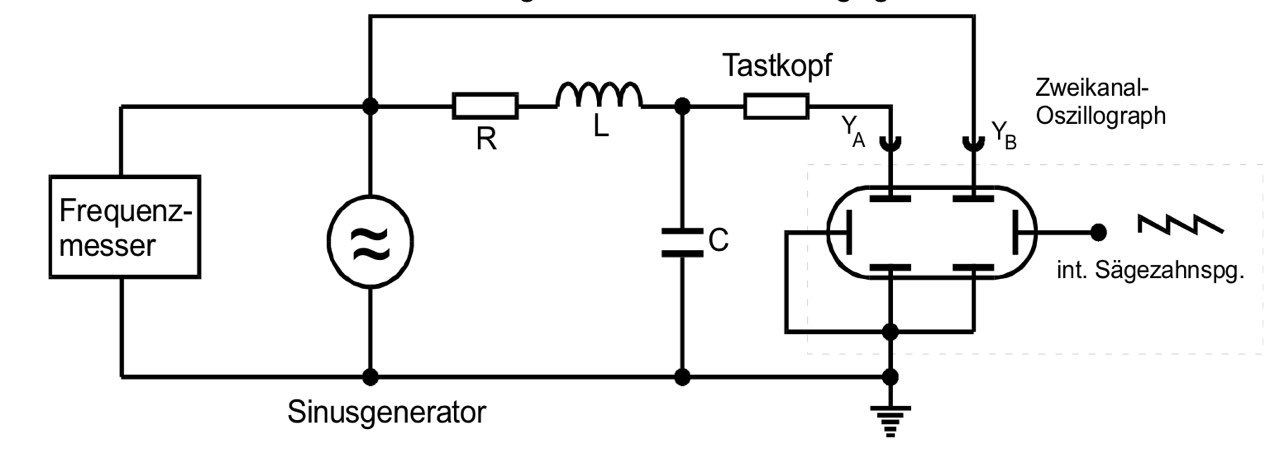
\includegraphics[width=0.6\textwidth]{bilder/Frequenzabhaengigkeit_Phase.jpeg}
    \caption{Versuchsaufbau - Frequenzabhängigkeit der Phasendifferenz}
    \label{fig:Aufbau3}
\end{figure}